%%%%%%%%%%%%%%%%%%%%%%%%%%%%%%%%%%%%%%%%%
% Lachaise Assignment
% LaTeX Template
% Version 1.0 (26/6/2018)
%
% This template originates from:
% http://www.LaTeXTemplates.com
%
% Authors:
% Marion Lachaise & François Févotte
% Vel (vel@LaTeXTemplates.com)
%
% License:
% CC BY-NC-SA 3.0 (http://creativecommons.org/licenses/by-nc-sa/3.0/)
% 
%%%%%%%%%%%%%%%%%%%%%%%%%%%%%%%%%%%%%%%%%

%----------------------------------------------------------------------------------------
%	PACKAGES AND OTHER DOCUMENT CONFIGURATIONS
%----------------------------------------------------------------------------------------

\documentclass{article}
\usepackage{float}
%%%%%%%%%%%%%%%%%%%%%%%%%%%%%%%%%%%%%%%%%
% Lachaise Assignment
% Structure Specification File
% Version 1.0 (26/6/2018)
%
% This template originates from:
% http://www.LaTeXTemplates.com
%
% Authors:
% Marion Lachaise & François Févotte
% Vel (vel@LaTeXTemplates.com)
%
% License:
% CC BY-NC-SA 3.0 (http://creativecommons.org/licenses/by-nc-sa/3.0/)
% 
%%%%%%%%%%%%%%%%%%%%%%%%%%%%%%%%%%%%%%%%%

%----------------------------------------------------------------------------------------
%	PACKAGES AND OTHER DOCUMENT CONFIGURATIONS
%----------------------------------------------------------------------------------------

\usepackage{amsmath,amsfonts,stmaryrd,amssymb} % Math packages

\usepackage{enumerate} % Custom item numbers for enumerations

\usepackage[ruled]{algorithm2e} % Algorithms

\usepackage[framemethod=tikz]{mdframed} % Allows defining custom boxed/framed environments

\usepackage{listings} % File listings, with syntax highlighting
\lstset{language=C,keywordstyle={\bfseries \color{blue}}}

%----------------------------------------------------------------------------------------
%	DOCUMENT MARGINS
%----------------------------------------------------------------------------------------

\usepackage{geometry} % Required for adjusting page dimensions and margins

\geometry{
	paper=a4paper, % Paper size, change to letterpaper for US letter size
	top=2.5cm, % Top margin
	bottom=3cm, % Bottom margin
	left=2.5cm, % Left margin
	right=2.5cm, % Right margin
	headheight=14pt, % Header height
	footskip=1.5cm, % Space from the bottom margin to the baseline of the footer
	headsep=1.2cm, % Space from the top margin to the baseline of the header
	%showframe, % Uncomment to show how the type block is set on the page
}

%----------------------------------------------------------------------------------------
%	FONTS
%----------------------------------------------------------------------------------------

\usepackage[utf8]{inputenc} % Required for inputting international characters
\usepackage[T1]{fontenc} % Output font encoding for international characters

\usepackage{XCharter} % Use the XCharter fonts

%----------------------------------------------------------------------------------------
%	COMMAND LINE ENVIRONMENT
%----------------------------------------------------------------------------------------

% Usage:
% \begin{commandline}
%	\begin{verbatim}
%		$ ls
%		
%		Applications	Desktop	...
%	\end{verbatim}
% \end{commandline}

\mdfdefinestyle{commandline}{
	leftmargin=10pt,
	rightmargin=10pt,
	innerleftmargin=15pt,
	middlelinecolor=black!50!white,
	middlelinewidth=2pt,
	frametitlerule=false,
	backgroundcolor=black!5!white,
	frametitle={Command Line},
	frametitlefont={\normalfont\sffamily\color{white}\hspace{-1em}},
	frametitlebackgroundcolor=black!50!white,
	nobreak,
}

% Define a custom environment for command-line snapshots
\newenvironment{commandline}{
	\medskip
	\begin{mdframed}[style=commandline]
}{
	\end{mdframed}
	\medskip
}

%----------------------------------------------------------------------------------------
%	FILE CONTENTS ENVIRONMENT
%----------------------------------------------------------------------------------------

% Usage:
% \begin{file}[optional filename, defaults to "File"]
%	File contents, for example, with a listings environment
% \end{file}

\mdfdefinestyle{file}{
	innertopmargin=1.6\baselineskip,
	innerbottommargin=0.8\baselineskip,
	topline=false, bottomline=false,
	leftline=false, rightline=false,
	leftmargin=2cm,
	rightmargin=2cm,
	singleextra={%
		\draw[fill=black!10!white](P)++(0,-1.2em)rectangle(P-|O);
		\node[anchor=north west]
		at(P-|O){\ttfamily\mdfilename};
		%
		\def\l{3em}
		\draw(O-|P)++(-\l,0)--++(\l,\l)--(P)--(P-|O)--(O)--cycle;
		\draw(O-|P)++(-\l,0)--++(0,\l)--++(\l,0);
	},
	nobreak,
}

% Define a custom environment for file contents
\newenvironment{file}[1][File]{ % Set the default filename to "File"
	\medskip
	\newcommand{\mdfilename}{#1}
	\begin{mdframed}[style=file]
}{
	\end{mdframed}
	\medskip
}

%----------------------------------------------------------------------------------------
%	NUMBERED QUESTIONS ENVIRONMENT
%----------------------------------------------------------------------------------------

% Usage:
% \begin{question}[optional title]
%	Question contents
% \end{question}

\mdfdefinestyle{question}{
	innertopmargin=1.2\baselineskip,
	innerbottommargin=0.8\baselineskip,
	roundcorner=5pt,
	nobreak,
	singleextra={%
		\draw(P-|O)node[xshift=1em,anchor=west,fill=white,draw,rounded corners=5pt]{%
		Question \theQuestion\questionTitle};
	},
}

\newcounter{Question} % Stores the current question number that gets iterated with each new question

% Define a custom environment for numbered questions
\newenvironment{question}[1][\unskip]{
	\bigskip
	\stepcounter{Question}
	\newcommand{\questionTitle}{~#1}
	\begin{mdframed}[style=question]
}{
	\end{mdframed}
	\medskip
}

%----------------------------------------------------------------------------------------
%	WARNING TEXT ENVIRONMENT
%----------------------------------------------------------------------------------------

% Usage:
% \begin{warn}[optional title, defaults to "Warning:"]
%	Contents
% \end{warn}

\mdfdefinestyle{warning}{
	topline=false, bottomline=false,
	leftline=false, rightline=false,
	nobreak,
	singleextra={%
		\draw(P-|O)++(-0.5em,0)node(tmp1){};
		\draw(P-|O)++(0.5em,0)node(tmp2){};
		\fill[black,rotate around={45:(P-|O)}](tmp1)rectangle(tmp2);
		\node at(P-|O){\color{white}\scriptsize\bf !};
		\draw[very thick](P-|O)++(0,-1em)--(O);%--(O-|P);
	}
}

% Define a custom environment for warning text
\newenvironment{warn}[1][Warning:]{ % Set the default warning to "Warning:"
	\medskip
	\begin{mdframed}[style=warning]
		\noindent{\textbf{#1}}
}{
	\end{mdframed}
}

%----------------------------------------------------------------------------------------
%	INFORMATION ENVIRONMENT
%----------------------------------------------------------------------------------------

% Usage:
% \begin{info}[optional title, defaults to "Info:"]
% 	contents
% 	\end{info}

\mdfdefinestyle{info}{%
	topline=false, bottomline=false,
	leftline=false, rightline=false,
	nobreak,
	singleextra={%
		\fill[black](P-|O)circle[radius=0.4em];
		\node at(P-|O){\color{white}\scriptsize\bf i};
		\draw[very thick](P-|O)++(0,-0.8em)--(O);%--(O-|P);
	}
}

% Define a custom environment for information
\newenvironment{info}[1][Info:]{ % Set the default title to "Info:"
	\medskip
	\begin{mdframed}[style=info]
		\noindent{\textbf{#1}}
}{
	\end{mdframed}
} % Include the file specifying the document structure and custom commands

%----------------------------------------------------------------------------------------
%	ASSIGNMENT INFORMATION
%----------------------------------------------------------------------------------------

\title{CS426: Project \#2 Report} % Title of the assignment

\author{Doruk Çakmakçı\\ \texttt{21502293}} % Author name and email address

\date{Bilkent University --- \today} % University, school and/or department name(s) and a date

%----------------------------------------------------------------------------------------

\begin{document}

\maketitle % Print the title

%----------------------------------------------------------------------------------------
%	INTRODUCTION
%----------------------------------------------------------------------------------------

\section{Main Program} % Unnumbered section
\qquad In this project, we implemented a parallel document search system using an algorithm similar to a simplified supervised search. In the system implemented, each document i is represented with a weight vector $w_{i}$. A weight vector is composed of D number of elements such that each of the weight values correspond to the relationship between file i and word j in our dictionary of size D. At the same time some queries are inserted to the system. Query is vector q which is composed of D integers. Then, the similarity values for each document and a query is calculated using the formula given in the project description. The output of our program is the K documents which are least related to the inserted query. The program consists of a serial part and a parallel part. The document and query fle reading operations are included in serial part, kreduce and preprocessing for the kreduce function are contained in the parallel part. \\
\null \qquad Since the query and the documents are given to the program as text files, utils.c handles the file IO part of our program. The query and documents are read line by line and a heap object for the two variables are created during file IO part of the serial execution. the outpur of reading files are an array that holds document ids, a multidimensional array that holds the document themselves and an array that holds the query. As a last minute note before submission: I found out that even though MPI\_Init function is used in the middle of the main function, the processes are still created at the start of the main function. So actually if the program is run with p processors and the document file and query file is read p times concurrently. To alter the program so that master is the only process that reads the file, MPI\_Init must be moved to the first lines of the main function along with MPI\_Comm\_rank and MPI\_Comm\_size calls. if the rank is 0, the master process reads the file and creates corresponding variables. Also, since the collective communication operations are banned outside of kreduce function, the master process must send the created variables to slave processes using one-to-one-communication operations of MPI. But note that even though the program is not written in this manner, the serial runtime difference should be negligible since the only difference between the two cases is the concurrent read operation done on the query and document files. There may be a negligible time difference between only master reading the files and all processors reading the files due to OS semaphores(or mutex locks, whichever is used). The printed serial time at the end on the main program is the time calculated for the master processor, not the average time nor the minimum time of the processors\\
\null \qquad The parallel part of the program, the only communication operations are done in kreduce function. The input to the parallel part of the program are the document ids, documents themselves and the query. First, each process computes how many documents to process and generate similarity values. the computation size depends on how many processes used and the size of the documents. Every process computes the similarity of the document in their portion to the query. Since the inputs of the kreduce function is fixed(myids and myvals array are K sized and sorted in ascending order according to their similarity values), a preprocessing is required to fit the computation size number of documents to the kreduce function. Since the relative order of document ids and similarity values must remain same after sorting, a pair is generated for each document that holds document id, similarity value and the rank of the processor that processed the document(needed for my kreduce implementation). The pairs are stored in an array and sorted using the quicksort implementation of C(qsort). qsort is used for the program in order not to reinvent the wheel even though radix sort may have smaller asymptotic runtime. Then the sorted result is disengaged to myids and myvals arrays. However, if the computation size is smaller than the value of K, then K - computation size elements of myvals array are filled with maximum integer values in order not to interrupt with the least k similar document generation. Else if the computation size is larger than K, the document array is truncated to K values and computation size - K documents are discarded since they can not be in the least K similar documents. After these operations, kreduce operation is called and the K documents that are least related to the  input query are returned using the parameter list. the ids of the documents are printed to the console along with the serial execution time and parallel execution time in milliseconds.
\section{Kreduce Function}
\qquad Before the explanation of my kreduce implementation the following preliminary information must be mentioned:
\begin{itemize}
    \item \textbf{Pair:} is a struct that holds document id, corresponding similarity value and the rank of the processor that processed the document to generate the similarity value. This processor also contains this document. 
    \item \textbf{MPI\_Op:} is an MPI library function that is used to generate a reduction operation for a given C function that compares any two reduced structs.
    \item \textbf{Generating User-Defined Reduce Operation For Finding Min Pair:} For the MPI\_Reduce operation used in the kreduce implementation that is generated using a C function that compares any two Pair structs based on their similarity value and MPI\_Op function. The C function also checks if the pairs compared are valid by checking if their ids equal to -1(-1 is an invalid id). There may be a situation where one or both of the compared pairs are invalid. I couldn't find a way to dynamically shrink or grow a communicator group. Therefore needed to handle the case where processors that only have invalid pairs reduce (all members of a communicator must be present and execute the reduce function. In other words, MPI\_reduce is blocking).
\end{itemize}
\null \qquad The first operation in the kreduce function is MPI\_Barrier to synchronize each process to the same point in their execution path. Then each process creates the reduction operation for upcoming reduction operations. Now each processor has a reduction operation, two arrays of size k in ascending order with respect to the similarity values(not ids) for document similarity values and ids respectively. Observe that the data for the minimum similarity valued document for each process is hold in the  first elements of the two arrays. Therefore, an index variable is created for each process that points to the location of the minimum similarity valued document in the two arrays. Then each process, including the master process, allocated data from the heap to store the hold the data for the pair under consideration. Master process uses an additional space in order to store the result of the reduction operation, the pair with the minimum similarity value. \\
\null \qquad Since we need  K least similar documents to the given query, K reduction operations are done during a kreduce function execution. After a reduction operation, master needs to notify the process who had the minimum similarity valued document to update their index to the next minimum value. Therefore, The master process broadcasts the rank of the processor which had the minimum pair and the corresponding process increments the index variable. However, there is an edgecase: if the two arrays are underfull, the two input arrays contain invalid elements. The pair comparison reduction operation handles this case by explicitly checking invalidity of the pairs. As mentioned before, if I could find a way to dynamically change the size of a communicator group, then the communication amount would decrease with respect to increasing iteration count. Also at the end of an iteration, there exists an MPI\_Barrier to synchronize the processes.\\
\null \qquad In total, for a single call of kreduce operation, K reduction operations and K broadcast operating are done. Note that a single integer is broadcasted by master process and a pair consisting 3 integers are reduced in an iteration. Also, the pair comparison operation is written in such a way that the intermediate step message size for the reduction operation becomes constant. As an analogy, the kreduce operation works similar to a K-way merge operation of K-mergesort, which stops after finding K smallest elements. Its time complexity is a factor of $ O( K( 1 + T(MPI\_Broadcast(int)) + T(MPI\_Reduce(3 * int)) ) )$. Its space requirement is rather small since all pairs are not preallocated but one current pair and one minimum pair is manipulated during execution.

\section{Parameters}
\qquad Many parameters affect the execution of this program such as current state of the processor and memory on a local computer, input size(how many documents are processed), output size( K  parameter),  dictionary size (D parameter), number of processes used for execution etc. However, the parameters under consideration are the following subsections. Note that in the submission folder, outputs folder contains the corresponding input document files query files. Also this folder contains several folders named same as the input files that contains outputs from different parameter settings. These runs are the basis for the figures in this section.
\subsection{Number of Processes}
\qquad Number of Processes is chosen as a parameter because varying processor size changes the amount of work done per processor drastically. In other words, for this problem, our goals are to determine if fine grain task decomposition or coarse grain task decomposition gives a better result, and if processing tasks of bigger size or creating new processes generate more overhead
\subsection{Number of Documents(Input Size)}
\qquad Number of Documents is chosen as a parameter because, as we also observed in project 1, larger input size changes program running time drastically. We seek to show the relationship between input size and program runtime.
\subsection{K(Output Size)}
\qquad Output Size(K) is chosen as a parameter because k determines the running time of kreduce function and therefore it is used to analyze kreduce function runtime.
\subsection{Dictionary Size(D)}
\qquad Dictionary size(D) is chosen as a parameter because it changes the running time of the code snippet for similarity value computation. Also from another perspective, input is has two dimensions: number of documents and dictionary size.

\section{Graphs With Respect to Varying Parameters and Discussion}
\subsection{Number of Processes}

\begin{figure}[H]
\centering
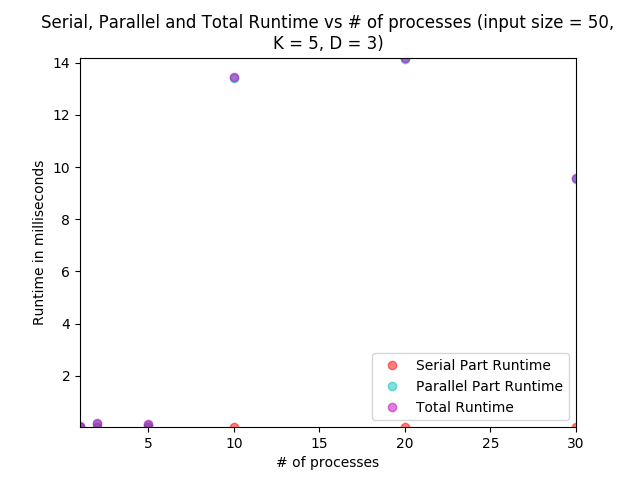
\includegraphics[width=\linewidth]{assets/input_size_50_K_5_D_3.png}
\label{fig:test1}
\vspace{-2pt}
\caption{Experiment while the number of processes is changed.}
\end{figure}

\subsubsection{Discussion}
\qquad It is seen that the runtime of the serial part of the program is not affected by the change in the number of processes used as much as the parallel part of the program. This is a maningful result since the serial part of the program is executed only by the master process and hence it is not affected by the number of processes. There are some minimal oscillations which are completely normal since the execution time of a program is also dependent to various factors. For example, the current state of the computer(since this program is run on a single computer, at least for this project) determines the memory IO time and master process runtime.\\
\null \qquad On the other hand, the parallel part of a program is highly dependent on the efficiency of the kreduce function and ultimately the number of processes used to execute the program. From the figure we see that for the number of processes $<= 5$, the runtime of the program is not increasing drastically. However, for the number of processes $>= 10$, we see that the parallel part of the program has much higher runtime than the other case. For the current controlled parameter values(K = 5, D = 3 and input size = 50), we can infer that using more than 5 processes creates an overhead due to excess process creation. So for this parameter setting, using 5 processes is highly feasible. Also, the number of process $ = 1 $ is the closest runtime setting to the parallel execution runtime however, in this case, the communication operations become the overhead that increases the runtime( due to the meaningless communication statements).\\
\null \qquad Lastly, since the total time is only the sum of the serial and parallel part runtimes, it is also subject to the same discussion for the serial and the parallel parts.

\subsection{Number of Documents(Input Size)}

\begin{figure}[H]
\centering\caption{Experiment while the output size is changed changed.}
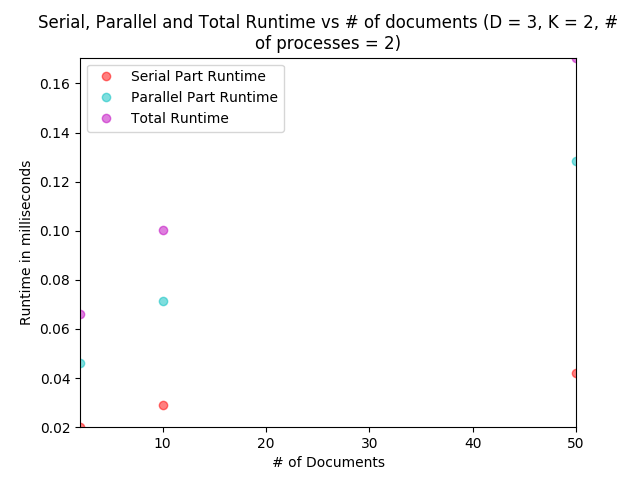
\includegraphics[width=\linewidth]{assets/D_3_K_2_numproc_2.png}
\label{fig:test1}
\vspace{-2pt}
\caption{Experiment while the number of documents is changed.}
\end{figure}

\subsubsection{Discussion}
\qquad The runtime of the serial part of this program is highly effected by the number of documents(since file operations are done as a read of the number of documents times lines). From the figure we see that the runtime of the serial part of the program is almost linearly proportional to the number of documents. The effect is not drastic here because the dictionary size is small. However, if the dictionary size was large, we would have observed a more steeper increase in the serial runtime.\\
\null \qquad The runtime of the parallel part of the program is also dependent to the number of documents. Each process finds the similarity value of  $ ( the number of documents )/( the number of processes )$. So when the number of documents are increased, each process does more work than the previous state of parameter values. \\
\null \qquad Overall, from the figure we can infer the the change in the runtime of the parallel part of the program is more than the change in the serial part of the program. The performance of the parallel part stays the same when the performance is calculated with respect to the input size. As before, the total time is the sum of the parallel and the serial time. Also note that for this runtime experiment, input size , the \# of processes and the dictionary size remains  constant(control variable); the runtime of the serial and the parallel parts are the dependent variables while the number of documents(independent variable) is changed.

\subsection{K(Output Size)}

\begin{figure}[H]
\centering
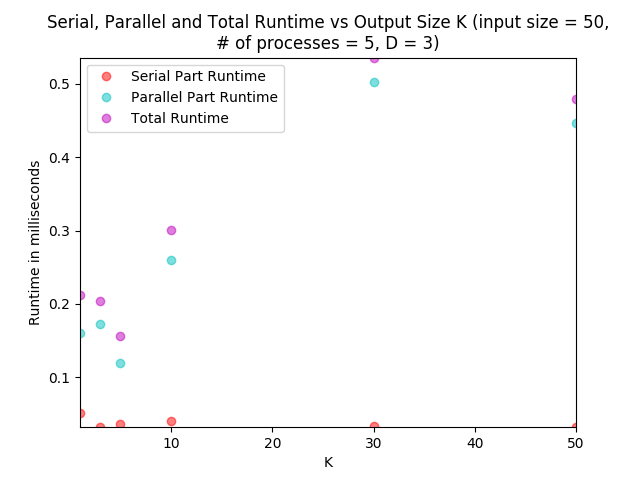
\includegraphics[width=\linewidth]{assets/input_size_50_numproc_5_D_3.png}
\label{fig:test1}
\vspace{-2pt}
\caption{Experiment while the output size is changed.}
\end{figure}

\subsubsection{Discussion}
\qquad In theory, the runtime of the serial part of this program should not be affected by the output size because the number of documents read and their dimensions are fixed. I think that the oscillations in the figure is due to the state of the computer while this program is run. \\
\null \qquad The runtime of the parallel part of the program highly dependent to the K number because, because kreduce implementation reduces and broadcasts items K times. We can state that generally when the value of K increases, the runtime of the parallel part of the program also increases. From the figure we can see that the runtime of the parallel part of the program corresponding to $K = 5$ is less than the runtime of the parallel part of the program corresponding to smaller K values. This occurence may be due to the coincidence or this result may be an outlier and should not affect our claim.. The interpretation for the total time is the same as the other parameters.

\subsection{D(Dictionary Size)}

\begin{figure}[H]
\centering
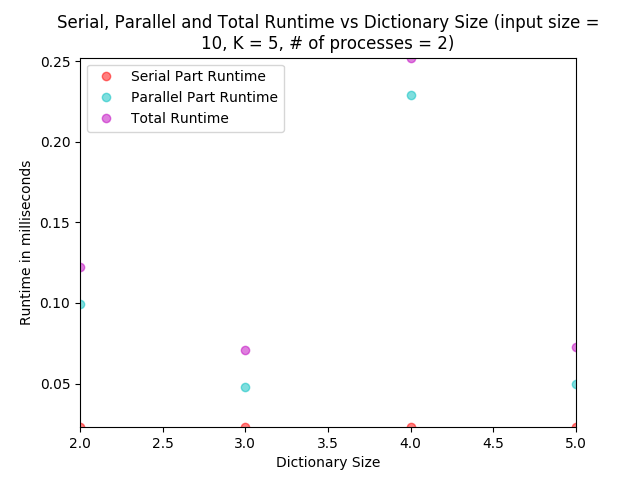
\includegraphics[width=\linewidth]{assets/input_size_10_K_5_numproc_2.png}
\label{fig:test1}
\vspace{-2pt}
\caption{Experiment while the dictionary size is changed.}
\end{figure}

\subsubsection{Discussion}
\qquad The document file consists of two dimensions: the dictionary size and the number of documents. If one of these dimensions is large, then a unit change in the other dimension would cause a drastic runtime change in the serial time. However, in this case, the numnber of documents is rather small. Therefore, it is normal that we do not observe a significant change in the serial time. For higher input sizes we will have seen a monotonic increase in the serial time.\\
\null \qquad The dictionary size has an effect on the calculation of the similarity values per processor and introduce an overhead. However, there are fluctuations in the paralel timing. This is due to the smallness of the input size. If the input size was significantly large, the state of the computer would be negligible since it would not introduce a significant change in the runtime. However in the mentioned case, the dictionary size would have introduced a slowdown rate that decreases when the current dictionary size is increased.
\end{document}
